
% !TeX spellcheck = de_DE
\documentclass{article}

\usepackage[ngerman]{babel}
\usepackage{graphicx}
\usepackage{indentfirst}
\usepackage{hyperref}
\usepackage{geometry}
\usepackage{changepage}

\graphicspath{ {./images/} }

\makeatletter
\newcommand{\sectionauthor}[1]{
	{\parindent 0em \large \scshape Autor: #1 \par \nobreak \vspace*{1em}}
	\@afterheading
}
\newcommand{\specification}[3]{
	{\parindent 0.5em \hangindent 3em \hypertarget{spec:#1:#2}{\textbf{/#1#2/}} #3 \par \nobreak \vspace*{0.5em}}
}
\makeatother

\begin{document}

%--Einleitung--------------------------------------------------------------------------------------------------------------------------------------------------------------------------
\section{Einleitung}
\sectionauthor{Jonas Picker}
Hier wird der Entwurf des Bibliotheksmanagementsystems BiBi beschrieben. Das Dokument bezieht sich auf das Lastenheft von Christian Bachmaier und Armin Größlinger und stellt eine technische Vertiefung unseres Pflichtenhefts dar, welches im Folgenden wiederholt referenziert wird. 

%--Systemarchitektur---------------------------------------------------------------------------------------------------------------------------------------------------------------
\section{Systemarchitektur}
\sectionauthor{Ivan Charviakou}

%--Klassendiagramm---------------------------------------------------------------------------------------------------------------------------------------------------------------
\section{Klassendiagramm}
\sectionauthor{Mohamad Najjar}

%--JSF-Dialoge-----------------------------------------------------------------------------------------------------------------------------------------------------------------------
\section{JSF-Dialoge}
\sectionauthor{León Liehr}

%--Systemfunktionen----------------------------------------------------------------------------------------------------------------------------------------------------------------
\section{Systemfunktionen}
\sectionauthor{Jonas Picker}
\subsection{Technische Systemsicherheit}
\noindent \textbf{Kommunikationsverschlüsselung:} Durch das vorrausgesetzte SSL-Zertifikat des Tomcat-Servers wird der Anwendung die Kommunikation mit dem HTTPS-Protokoll ermöglicht. Dies ist eine Ergänzung der HTTP-Kommunikation um eine Transportverschlüsselung. Zusätzlich zur Vereitelung von Abhörversuchen der an Ihren Server gesendeten Anfragen signalisieren Sie den Klienten so auch die Vertrauenswürdigkeit Ihrer Institution durch die CA\footnote{'Certification Authority' - eine digitale Zertifizierungsstelle}-Zertifizierung.\\
\textbf{Nutzerberechtigungen:} Um zu Verhindern, dass Nutzer ohne ausreichende Berechtigungen auf zugangsbeschränkte Bereiche des Webspaces zugreifen können, werden entsprechende Maßnahmen ergriffen: Um den direkten Aufruf von Seiten, die für den Nutzer nicht zugänglich sein sollten, zu unterbinden, verwenden wir einen sogenannten Phaselistener. Wie jede JSF-Anwendung durchläuft auch unsere nach Erhalt einer Anfrage eine Reihe von Verarbeitungsphasen, bevor die Antwort an den Klienten fertiggestellt und verschickt wird. Ein Phaselistener kann während dieses Prozesses zusätzliche Integritätsbedingungen abprüfen und gegebenenfalls die Antwort auf die Anfrage verändern/verhindern. Zusätzlich wird durch das in JSF eingebaute Session-Tracking\footnote{Das Verfolgen der Klientenverbindung zwischen den eigentlich verbindungslosen HTTP-Anfragen} sichergestellt, dass die verschiedenen Nutzerrollen eine unterschiedliche Version der gleichen Seiten angezeigt bekommen, deren Funktionalitäten den Berechtigungen der Rollen entsprechen. Es wird durch das manuelle Austauschen des Identifikators für die Nutzer-Session an kritischen Stellen dafür gesorgt, dass Nutzer vor Session-Hijacking\footnote{Das Stehlen einer validen Nutzer-Session um Zugriff auf den Account und seine Berechtigungen zu erhalten} geschützt werden.\\
\textbf{Vorbeugen von Angriffen:} Durch geschicktes Einschleusen von SQL\footnote{'Structured Query Language' - eine weit verbreitete Datenbankanfragesprache}-Code in ungesicherte Formularfelder könnten Unbefugte direkten Zugriff auf die darunterliegende Datenbank erhalten. Der Datenbankzugriff in unserem System erfolgt via JDBC\footnote{'Java Database Connectivity' - eine universelle Datenbankschnittstelle}, welche bereits über einen Mechanismus zur Verhinderung von diesen SQL-Injections verfügt. Hierbei wird verhindert, dass von Nutzern eingegebener Text vom Managementsystem der Datenbank interpretiert wird. Ein weiterer Angriffsvektor stellt das sogenannte Cross-Site-Scripting dar. Dabei wird versucht, nutzergenerierte Teile von Websiten mit vom Browser interpretierbaren Codeabschnitten zu füllen, welche dann beim Anzeigen des Inhalts bei anderen Klienten ausgeführt werden. Es gibt verschiedene Versionen dieser Angriffsart, von denen nicht alle am Server verhindert werden können. Jedoch wird in der Anwendungslogik jede Nutzereingabe auf interpretierbaren HTML (und eingebundenen JavaScript) Code untersucht und gegebenenfalls entschärft.
\subsection{Fehlerbehandlung und Logging}
Von uns vorhergesehene Fehler und einige im Hintergrund ablaufende Prozesse werden durch einen selbst erstellten Logging-Mechanismus dokumentiert. Da dieser Mechanismus während des Entwicklungsprozesses ebenfalls nützlich ist und auf feinster Einstellung für den Anwender uninteressant sein könnte, wird es eine Option geben, die den Detailgrad und die Anzahl der ausgegebenen Meldungen festlegt. Alle Meldungen werden in eine seperate Log-Datei geschrieben und können wahlweise auf der Konsole angezeigt werden. Vorhergesehene Fehler in Abläufen werden von der Anwendung bestmöglich abgehandelt und wie erwähnt durch das Logging dokumentiert/kommuniziert. Sollte jedoch ein nicht vorhergesehener Fehler auftreten, wird der Grund dafür in Form der Java-eigenen Exceptions auf die Konsole ausgegeben. Durch umfangreiches Testen der Anwendung vor Auslieferung versuchen wir, solche Fehlerquellen zu finden und zu beheben. Im Optimalfall kommen Sie nicht mit unvorhergesehen Fehlern in Berührung. Sollten sie dennoch auftreten, wenden Sie sich bitte direkt an uns.
\subsection{Selbstständige Prozesse}
Im System gibt es verschiedene Fristen (Abholungsmarkierung, Ausleihrückgabe [global, pro Medium, pro Nutzer], Gültigkeit des Verifizierungs-/Zurücksetzungslinks, Mahnungszeitversatz) und damit verbundene Aktionen. Um diese Aktionen ausführen zu können, muss das System in gewissen Abständen selbstständig auf die Datenbank zugreifen. In der Klasse ???? ist dafür ein eigener Wartungsthread implementiert.
\subsection{Starten und Stoppen der Anwendung}
\noindent \textbf{Start:} Beim Systemstart wird zunächst der oben beschriebene Logging-Mechanismus initialisiert. Im Anschluss liest das System die Konfigurationsdatei ein und versucht die dort angegebene Verbindung zur Datenbank. Bei erfolgreicher Verbindung wird überprüft, ob die benötigten Tabellennamen alle existieren bzw. legt diese bei deren Fehlen an. Sollte die Struktur der Tabellen fehlerhaft sein, wird eine Fehlermeldung geloggt und die Tabellen werden nicht vom System benutzt. Wenn die Datenbank fehlerhaft/nicht verbunden ist, werden eingehende Anfragen mit einer Fehlerseite beantwortet. Nach erfolgreichem Ablauf der vorhin genannten Prozesse wird als nächstes der Wartungsthread angestoßen, um fristenabhängige Aktionen durchzuführen. Danach ist das System vollständig betriebsbereit.\\
\textbf{Stop:} 
Beim planmäßigen Herunterfahren des Systems werden zunächst die noch offenen Datenbankverbindungen geschlossen und danach die Anwendung gestoppt. Dda dies sehr schnell passiert, wird währenddessen auf eine extra Umleitung der Nutzer auf eine Fehlerseite verzichtet. Da unsere SQL-Transaktionen dem ACID\footnote{'Atomicity, Consistency, Isolation, Durability' - ein Leitsatz von Eigenschaften für Datenbanktransaktionen}-Prinzip folgen, wird die Datenbank jedoch auch beim Herunterfahren während eines Zugriffs in konsistentem Zustand hinterlassen. Nutzersessions überleben das Ausschalten des Servers nicht, d.h. alle eingeloggten Nutzer sind nach einem Neustart des Systems ausgeloggt. Wenn die Java Laufzeitumgebung des Systems plötzlich beendet wird und das System abstürzt, wird mittels einer sogenannten ShutdownHook trotzdem noch versucht, offene Datenbankverbindungen zu schließen. Dies ist bei einem Stromausfall allerdings unmöglich. 
%--Datenfluss--------------------------------------------------------------------------------------------------------------------------------------------------------------------------
\section{Datenfluss}
\sectionauthor{Sergei Pravdin}

%--ER-Modell--------------------------------------------------------------------------------------------------------------------------------------------------------------------------
\section{ER-Modell}
\sectionauthor{Jonas Picker}

\newpage
\newgeometry{left=0cm,right=0cm,top=0cm,bottom=0cm}

\begin{figure}[h]
    \centering
    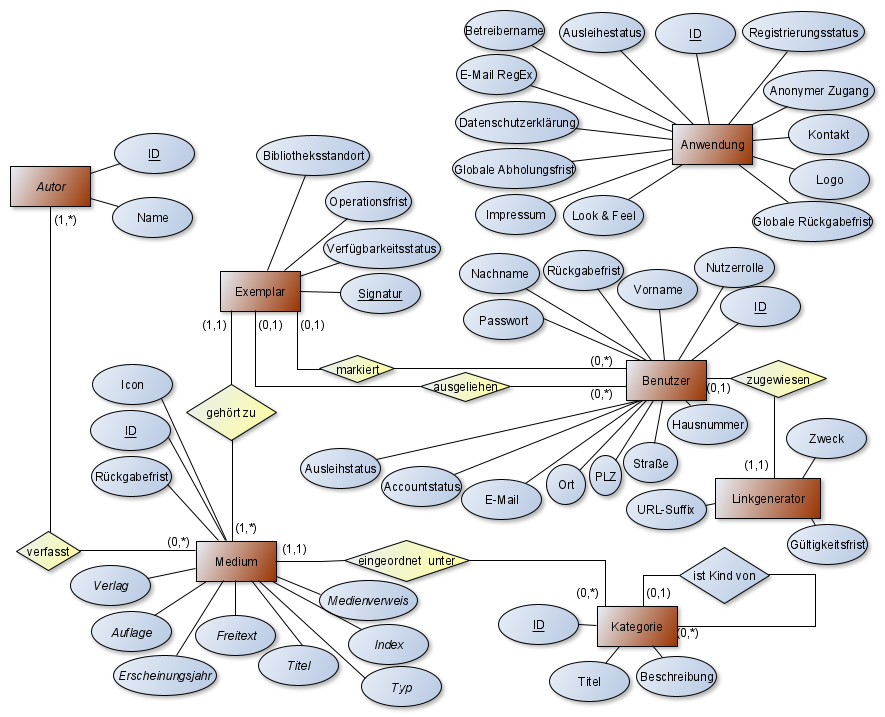
\includegraphics[angle = 270, width = 60em]{ER-Diagramm}
    \caption{Entity-Relationship Diagramm}
    \label{ER-Diagramm}
\end{figure}

\restoregeometry
\newpage

\subsection{Legende}
Jede Entität wird im Folgenden zusammen mit ihren nicht offensichtlichen Attributen und Relationen kurz beschrieben.\\
\textbf{Medium:} Diese Entität modelliert die in der Bibliothek gehaltenen Medien. Zusätzlich zum Primär-schlüssel ist auch das Attribut 'Rückgabefrist' und 'Icon' nicht vom Administrator entfernbar, die restlichen Attribute (kursiv) stellen den modifizierbaren Standartsatz der Medienattribute dar (PfHft. /D020/). Erwähnenswert ist hier noch das als mehrwertig markierte, editierbare Attribut 'Autoren', diese Markierung kann auch zu benutzerdefinierten Attributen hinzugefügt werden und wird mit dem Anlegen einer neuen Entität modelliert (PfHft. /F380/).\\
\textbf{Kategorie:} Die mit dieser Entität verbundenen Relationen ordnen jedem Medium genau eine Kategorie zu und modellieren die Kategoriehierarchie (PfHft. /W440/) durch die Selbstbeziehung. Es wird einen unlöschbaren Top-Knoten in der Hierarchie geben, zu dem alle Medien, die nie in eine Kategorie eingeteilt wurden oder deren Kategorie gelöscht wurde, gehören. Sollten alle Medien in benutzerdefinierten Kategorien stecken, hat der Top-Knoten keine zugeordneten Medien und nimmt somit nicht an der 'eingeordnet unter'-Relation teil.\\
\textbf{Exemplar:} Von jedem Medium muss mindestens ein Exemplar vorhanden sein. Auch kann ein bestimmtes Exemplar von genau einem Nutzer zur Abholung markiert oder ausgeliehen werden, diese Aktionen schließen sich gegenseitig aus (PfHft. /F310/) und ändern (genau wie eine Rückgabe) den Verfügbarkeitsstatus und die dazugehörige Operationsfrist dementsprechend. \\
\textbf{Benutzer:} Ob ein Benutzer die Ausleihfunktion benutzen kann, wird durch das Attribut 'Ausleihstatus' modelliert. 'Accountstatus' zeigt hingegen an, ob der Nutzeraccount bereits den Verifizierungsprozess durchlaufen hat (PfHft. /W70/). Das Passwort wird in gehashter Form abgespeichert. \\
\textbf{Linkgenerator:} Diese Entität kapselt einen befristet gültigen URL-Suffix, aus dem der Verifizierungs- oder Passwortzurücksetzungslink (je nach Zweck) für genau einen Account erstellt wird.\\
\textbf{Anwendung:} Hier werden die setzbaren globalen Variablen und Anwendungseinstellungen gespeichert. Diese Tabelle hat nur einen einzigen Eintrag. 'Anonymer Zugang' modelliert die Berechtigungen anonymer Nutzer beim Besuchen des Webspaces (PfHft. /F10/), während 'Registrierungsstatus' eine nutzerfreundlichere Alternative als den RegEx zum Sperren der Registrierung bietet (PfHft. /F20/). 'Ausleihstatus' steht für das Umschalten des Systems zur manuellen Freischaltung der Ausleihfunktion für registrierter Nutzer. 'Look \& Feel' speichert das momentan ausgewählte Farbschema. \\

\end{document}

